\section{Exercise 5: Optimization of the decoupling capacitors}

In this last exercise the five decoupling capacitors are connected to the package, and their values are chosen to minimise the peak-to-peak voltage ripple at the
die interface. Each of the five locations (C01--C05) can host one of the six vendor capacitors (1.5, 2.2, 3.3, 4.7, 6.8 and 10~nF), so there are
$6^5 = 7776$ possible configurations. Since a single transient simulation of the PDN takes about three minutes (Exercise~4), simulating all of them would require
more than two weeks. For this reason the problem is solved with a semi-analytical method: the PDN is characterised only once with a few AC
simulations, and the effect of any configuration of capacitors is then computed with simple matrix algebra.

%%%%%%%%%%%%%%%%%%%%%%%%%%%%%%%%%%%%%%%%%%%%%%%%%%%%%%%%%%%

\subsection{Impedance and voltage ripple with decoupling capacitors}
\label{sec:theory}

The PDN without decoupling capacitors, seen from the five capacitor locations and from the die, is a linear network with six ports: the ports $1,\dots,5$ at
the capacitor locations (C01--C05) and the port $d$ at the die interface. In the frequency domain, the network is described by its $6\times 6$ impedance matrix
$\mathbf{Z}(f)$, which links the port voltages to the port currents (all the currents flow \textit{into} the network):
\begin{equation}
  \begin{bmatrix} \mathbf{V}_c \\ V_d \end{bmatrix} =
  \begin{bmatrix} \mathbf{Z}_{cc} & \mathbf{Z}_{cd} \\ \mathbf{Z}_{dc} & Z_{dd} \end{bmatrix}
  \begin{bmatrix} \mathbf{I}_c \\ I_d \end{bmatrix},
  \label{eq:zmatrix}
\end{equation}
where $\mathbf{V}_c$ and $\mathbf{I}_c$ are the $5\times 1$ vectors of the voltages and of the currents at the capacitor ports, $\mathbf{Z}_{cc}$ is the
$5\times 5$ block between the capacitor ports, $\mathbf{Z}_{cd}$ and $\mathbf{Z}_{dc}$ are the $5\times 1$ and $1\times 5$ blocks that couple the capacitor
ports with the die port, and $Z_{dd}$ is the impedance seen from the die port when no capacitor is connected. The matrix is the one of the whole PDN, with the
VRM modelled as an ideal voltage source, which is a short circuit for the AC components, and with the passive RC network of the die.
Written out, the matrix equation \eqref{eq:zmatrix} becomes
\begin{align}
  \mathbf{V}_c &= \mathbf{Z}_{cc}\,\mathbf{I}_c + \mathbf{Z}_{cd}\,I_d, \label{eq:vc}\\
  V_d &= \mathbf{Z}_{dc}\,\mathbf{I}_c + Z_{dd}\,I_d. \label{eq:vd}
\end{align}

\noindent\\ When the capacitors are connected, each of them is a one-port connected between the capacitor port and the ground. The current that enters
the network is the opposite of the current that enters the capacitor, so that
\begin{equation}
  \mathbf{V}_c = -\mathbf{Z}_{cap}\,\mathbf{I}_c,
  \qquad
  \mathbf{Z}_{cap} = \mathrm{diag}\big(Z_{C_1}(f),\dots,Z_{C_5}(f)\big),
  \label{eq:cap}
\end{equation}
where $Z_{C_i}(f)$ is the impedance of the capacitor mounted on the location $i$, that is one of the six vendor models. Replacing \eqref{eq:cap} in
\eqref{eq:vc} gives
\begin{equation}
  -\mathbf{Z}_{cap}\,\mathbf{I}_c = \mathbf{Z}_{cc}\,\mathbf{I}_c + \mathbf{Z}_{cd}\,I_d
  \;\Longrightarrow\;
  \mathbf{I}_c = -\big(\mathbf{Z}_{cc} + \mathbf{Z}_{cap}\big)^{-1}\mathbf{Z}_{cd}\,I_d,
\end{equation}
which describes how the current injected at the die port is shared between the capacitors. Replacing this expression of $\mathbf{I}_c$ in \eqref{eq:vd}, the voltage
at the die port is
\begin{equation}
  V_d = \Big[ Z_{dd} - \mathbf{Z}_{dc}\big(\mathbf{Z}_{cc} + \mathbf{Z}_{cap}\big)^{-1}\mathbf{Z}_{cd} \Big] I_d ,
\end{equation}
and the impedance seen from the die with the decoupling capacitors, $Z_{die} = V_d/I_d$, is
\begin{equation}
  \boxed{\,Z_{die}(f) = Z_{dd}(f) - \mathbf{Z}_{dc}(f)\,\big[\mathbf{Z}_{cc}(f) + \mathbf{Z}_{cap}(f)\big]^{-1}\,\mathbf{Z}_{cd}(f)\,}
  \label{eq:zdie}
\end{equation}
This expression has the expected limits: if the capacitors are removed ($\mathbf{Z}_{cap}\to\infty$) the second term vanishes and $Z_{die} = Z_{dd}$, the
impedance of Exercise~2. Notice that the matrix $\mathbf{Z}$ is computed once, and only the diagonal matrix $\mathbf{Z}_{cap}$ changes when the configuration
changes, so \eqref{eq:zdie} can be evaluated for every configuration without any new simulation.

\noindent\\ The voltage ripple is obtained from the impedance and from the current drawn by the die. The PDN is linear and has only two independent sources:
the DC source of the VRM, which gives the constant part of the die voltage, and the load current $i_{load}(t)$ of the die model. By superposition, the
variation of the die voltage around its DC value is the response of the network to the load current alone. The die \textit{draws} the current $i_{load}$
from the supply, so the current that enters the network at the die port is $I_d = -I_{load}$, and the spectrum of the ripple is
\begin{equation}
  V_{rip}(f) = -\,Z_{die}(f)\;I_{load}(f).
  \label{eq:vrip}
\end{equation}
The current $i_{load}(t)$ is given by $N = 166\,664$ samples with a time step $\Delta t = 72~\text{ps}$, that is $12~\mu\text{s}$ in total. Its discrete
Fourier transform has lines at the frequencies
\begin{equation}
  f_k = k\,\Delta f, \qquad \Delta f = \frac{1}{N\,\Delta t} \simeq 83.33~\text{kHz},
\end{equation}
so \eqref{eq:vrip} is evaluated at each line $f_k$, with $I_{load}(f_k)$ equal to the DFT of the current. The ripple waveform in the time
domain is then the inverse transform of $V_{rip}(f_k)$, and the figure of merit used in the optimisation is its peak-to-peak value,
\begin{equation}
  V_{pp} = \max\{v_{rip}(t)\} - \min\{v_{rip}(t)\}
\end{equation}
The DC component is not included, since it does not change the peak-to-peak value. It should be noticed that the use of the DFT implicitly assumes that the
$12~\mu\text{s}$ current is repeated periodically, so $V_{pp}$ is the ripple of the periodic steady state: it does not contain the start-up transient that
appears at the beginning of a time-domain simulation.

%%%%%%%%%%%%%%%%%%%%%%%%%%%%%%%%%%%%%%%%%%%%%%%%%%%%%%%%%%%

\subsection{Characterisation of ports and capacitors: the 6+1 AC simulations}

The quantities needed by \eqref{eq:zdie} are obtained with seven AC simulations in LTspice, all of them using the same frequency grid $f_k = k\,\Delta f$, with
$k = 1,\dots,59\,999$. The grid is made of the harmonics of the $12~\mu\text{s}$ die current, so that the impedances are already available at the frequencies
where the current spectrum is defined, without any interpolation. The last line is at about $5~\text{GHz}$, the limit of validity of the board model
(Exercise~2).


\subsubsection{Six simulations for the impedance matrix.} Each column of $\mathbf{Z}(f)$ is measured by injecting a $1~\text{A}$ AC current at one port, leaving the other
five ports open: the voltages at the six ports are then equal to the impedances of the column, $Z_{ij} = V_i$ when the current is injected at the port $j$. The
netlists \texttt{zinj\_c01.cir}, \dots, \texttt{zinj\_c05.cir} and \texttt{zinj\_vdie.cir} are identical, except for the node of the current source (the capacitor
location or the die). Listing~\ref{lst:zinj} shows the netlist for the die port.

\begin{lstlisting}[language=ltspice, caption={\texttt{zinj\_vdie.cir} $\rightarrow$ injection of $1~\text{A}$ at the die port and extraction of one column of $\mathbf{Z}$.}, label={lst:zinj}]
.include "../eser1/pdn.cir"
Iinj 0 vdie DC 0 AC 1
.save V(c01) V(c02) V(c03) V(c04) V(c05) V(vdie)
.options numdgt=15
.ac lin 59999 83334.66668800035 4999996666.613333
.end
\end{lstlisting}

\noindent Only the six port voltages are saved, to keep the output files small, and the data are stored in double precision (\texttt{numdgt=15}). Since the network is
reciprocal, the matrix is symmetric ($\mathbf{Z}_{cd} = \mathbf{Z}_{dc}^{T}$), which has been used as a consistency check of the simulations.

%\noindent\\ \textbf{One simulation for the capacitors.} The impedance of the six vendor capacitors, $Z_{C}(f)$, is computed on the same grid in a single netlist
\subsubsection{One simulation for the capacitors.} The impedance of the six vendor capacitors, $Z_{C}(f)$, is computed on the same grid in a single netlist
(\texttt{caps\_zgrid.cir}). Each capacitor model is connected to ground, as in the PDN, and driven by its own $1~\text{A}$ AC current source, so that the voltage of each
node is the impedance of the capacitor, as in Exercise~3.

\noindent\\ In total, the characterisation requires seven AC simulations, each one lasting a few seconds. The first check of the method is the comparison with the
direct simulation of the PDN with the decoupling capacitors, described in \autoref{sec:best}.

%%%%%%%%%%%%%%%%%%%%%%%%%%%%%%%%%%%%%%%%%%%%%%%%%%%%%%%%%%

\subsection{Search of the optimal configuration}

The search is performed by the Python script \texttt{best\_decaps.py}, which reads the exported LTspice data (the six columns of $\mathbf{Z}$, the capacitor
impedances and the PWL die current), and applies the method of \autoref{sec:theory} to the $7776$ configurations. For each one it evaluates \eqref{eq:zdie} at
the frequency lines, applies \eqref{eq:vrip}, transforms back to the time domain and measures $V_{pp}$.

\noindent\\ To reduce the computation time, the first evaluation
uses only the frequency lines that hold $99.9\%$ of the power of the die current; the $300$ best candidates are then re-evaluated with all the
$59\,999$ lines. The whole search takes about two minutes, against the more than two weeks of the simulation of all the configurations. The result is written in a text file,
with the netlist lines of the best configuration ready to be pasted in the PDN netlist.

\noindent\\ The best configuration found is reported in \autoref{tab:best}. Its predicted ripple is $57.6~\text{mV}$, against $282.2~\text{mV}$ without decoupling capacitors. The
distribution of the ripple over all the configurations is shown in \autoref{fig:hist}: the median is about $82~\text{mV}$, and only a small fraction of the
configurations is close to the optimum. Moreover, many configurations are practically equivalent to the best one: about twenty of them are within $2\%$ of the optimal ripple, and the best ones
use only the 1.5, 2.2 and 3.3~nF capacitors. The smaller capacitors, with the higher self-resonance frequency, are therefore the best choice, and the largest
ones do not appear among the best configurations.

\begin{table}[!h]
\centering
\caption{Optimal configuration of the decoupling capacitors, and ripple predicted by the method of \autoref{sec:theory}.}
\label{tab:best}
\begin{tabular}{ccccc}
\hline
\textbf{C01} & \textbf{C02} & \textbf{C03} & \textbf{C04} & \textbf{C05} \\
\hline
3.3~nF & 2.2~nF & 1.5~nF & 1.5~nF & 2.2~nF \\
\hline
\end{tabular}
\end{table}

\begin{figure}[!h]
\centering
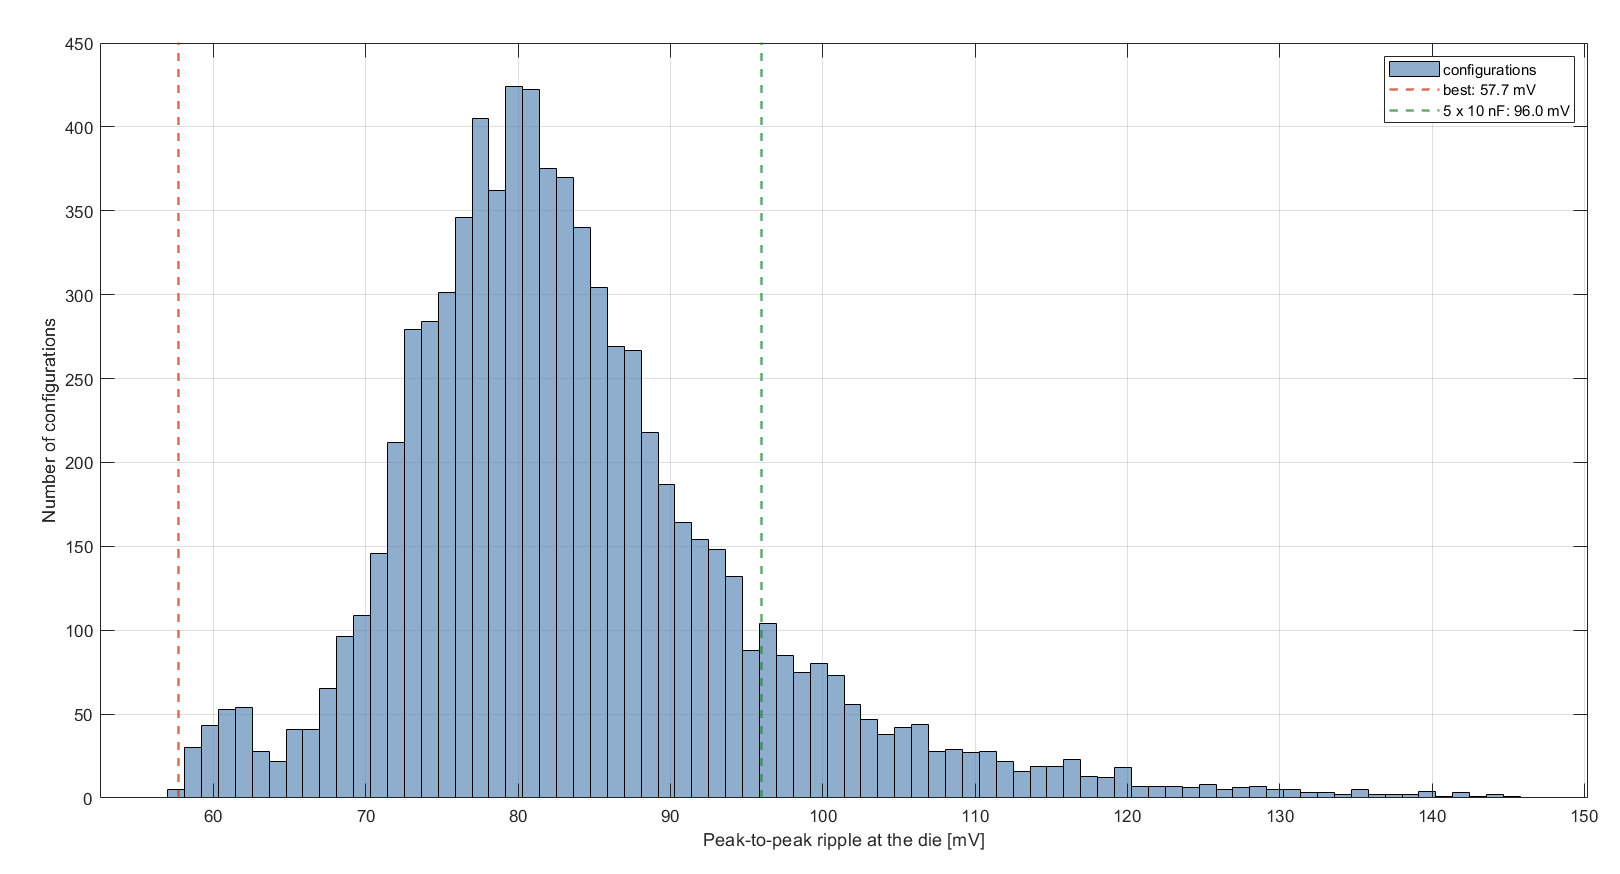
\includegraphics[width=0.8\textwidth]{./eser5/ripple_hist.png}
\caption{Distribution of the predicted peak-to-peak ripple over the 7776 configurations. The dashed lines show the optimal configuration and the configuration with five 10~nF capacitors.}
\label{fig:hist}
\end{figure}

\noindent The result also shows that the best configuration is not the one that gives the lowest peak of the impedance. The ripple depends on the impedance \textit{weighted by the
spectrum of the die current}, as in \eqref{eq:vrip}, and the spectrum is dominated by a line at $100~\text{MHz}$ (amplitude of about $56.5~\text{mA}$), with about $69\%$ of
the power between $50$ and $200~\text{MHz}$. The best configuration is the one that makes the impedance small exactly where the current is large: at $100~\text{MHz}$ the
impedance falls from $2.05~\Omega$ to $0.17~\Omega$, so the amplitude of the dominant line of the ripple falls from about $116~\text{mV}$ to about $10~\text{mV}$.

%%%%%%%%%%%%%%%%%%%%%%%%%%%%%%%%%%%%%%%%%%%%%%%%%%%%%%%%%%

\subsection{AC and transient analysis with the optimal decoupling capacitors}
\label{sec:best}

The optimal configuration has been verified with a direct simulation in LTspice, to check the predictions of the method. The netlists \texttt{pdn\_best\_ac.cir} and
\texttt{pdn\_best\_tran.cir} are the same ones of Exercises~2 and 4, with the five capacitors of \autoref{tab:best} added between the capacitor locations and the ground
(Listing~\ref{lst:best}).

\begin{lstlisting}[language=ltspice, caption={Connection of the optimal decoupling capacitors in the netlists \texttt{pdn\_best\_ac.cir} and \texttt{pdn\_best\_tran.cir}.}, label={lst:best}]
.include "../eser1/pdn.cir"
Xc01 c01 0 GCM033R71A332KA03      * 3.3nF
Xc02 c02 0 GCM033R71A222KA03      * 2.2nF
Xc03 c03 0 GCM033R71A152KA03      * 1.5nF
Xc04 c04 0 GCM033R71A152KA03      * 1.5nF
Xc05 c05 0 GCM033R71A222KA03      * 2.2nF
\end{lstlisting}

%\noindent\\ \textbf{Frequency domain.} The impedance seen from the die is shown in \autoref{fig:zdie_best}, together with the one of the PDN without decoupling capacitors.
\subsubsection{Frequency domain analysis of the PDN with optimal decaps configuration}
The impedance seen from the die with the optimal decaps configuration is shown in \autoref{fig:zdie_best}.\\
%together with the one of the PDN without decoupling capacitors.
The maximum of the impedance falls from $3.06~\Omega$ at $95.9~\text{MHz}$ to $0.829~\Omega$ at $74.9~\text{MHz}$ (the \texttt{.meas} of LTspice gives
$-1.63263~\text{dB}$). The resonance peak is therefore reduced by a factor of about $3.7$, and it is moved away from the $100~\text{MHz}$ line of the die current, where the impedance is now only
$0.17~\Omega$. The maximum and the frequency obtained from \eqref{eq:zdie} are the same ones of LTspice, which confirms that the matrix method reproduces the direct simulation.

\begin{figure}[!h]
\centering
% Replace the placeholder below with the LTspice plot (no decaps and optimal decaps on the same axes):
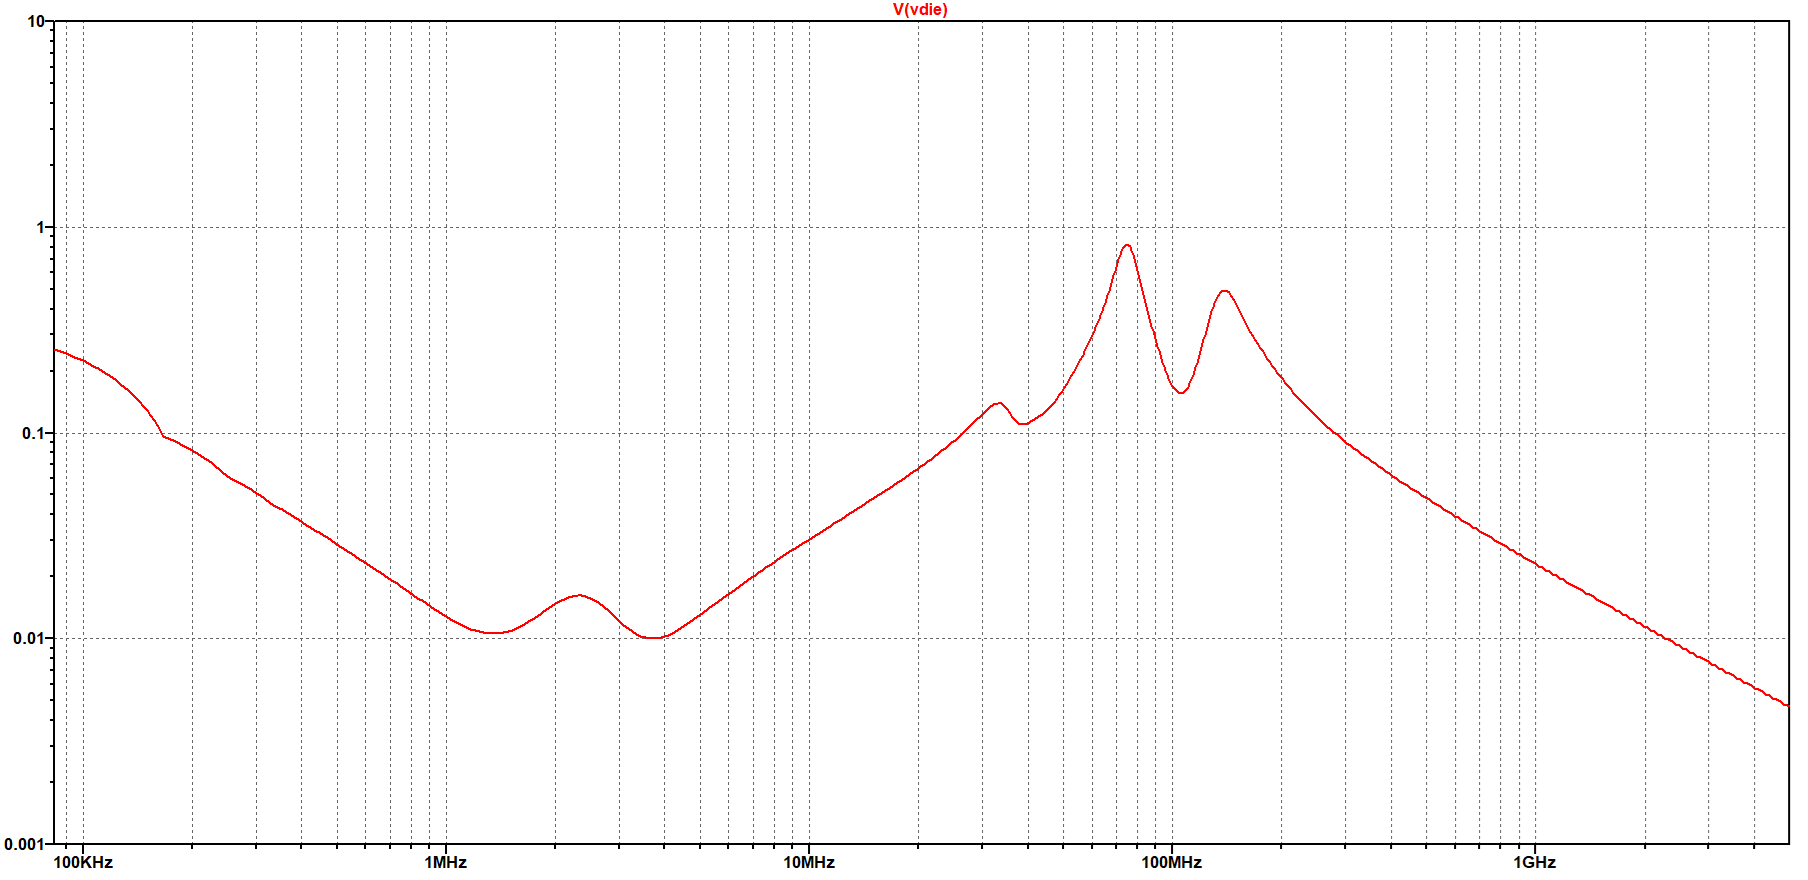
\includegraphics[width=0.95\textwidth]{./eser5/zdie_best.png}
%\fbox{\parbox{0.9\textwidth}{\centering\vspace{3cm} Figure placeholder: $|Z_{die}|$ without decoupling capacitors and with the optimal configuration\vspace{3cm}}}
\caption{Impedance magnitude seen from the die interface with optimal decaps configuration}
\label{fig:zdie_best}
\end{figure}

%\noindent\\ \textbf{Time domain.} The transient simulation uses the same settings of Exercise~4 ($12~\mu\text{s}$, maximum time step of $72~\text{ps}$). The
\subsubsection{Time domain simulation of the PDN with optimal decaps configuration} The transient simulation uses the same settings of Exercise~4 ($12~\mu\text{s}$, maximum time step of $72~\text{ps}$). The
peak-to-peak ripple measured by LTspice over the whole simulation is $59.5~\text{mV}$, against $280.8~\text{mV}$ of the PDN without decoupling capacitors: the ripple is reduced by about $79\%$, that is by a factor of $4.7$.
The waveform is shown in \autoref{fig:vdie_best}.

\begin{figure}[!h]
\centering
% Replace the placeholder below with the LTspice plot of V(vdie) with the optimal decaps:
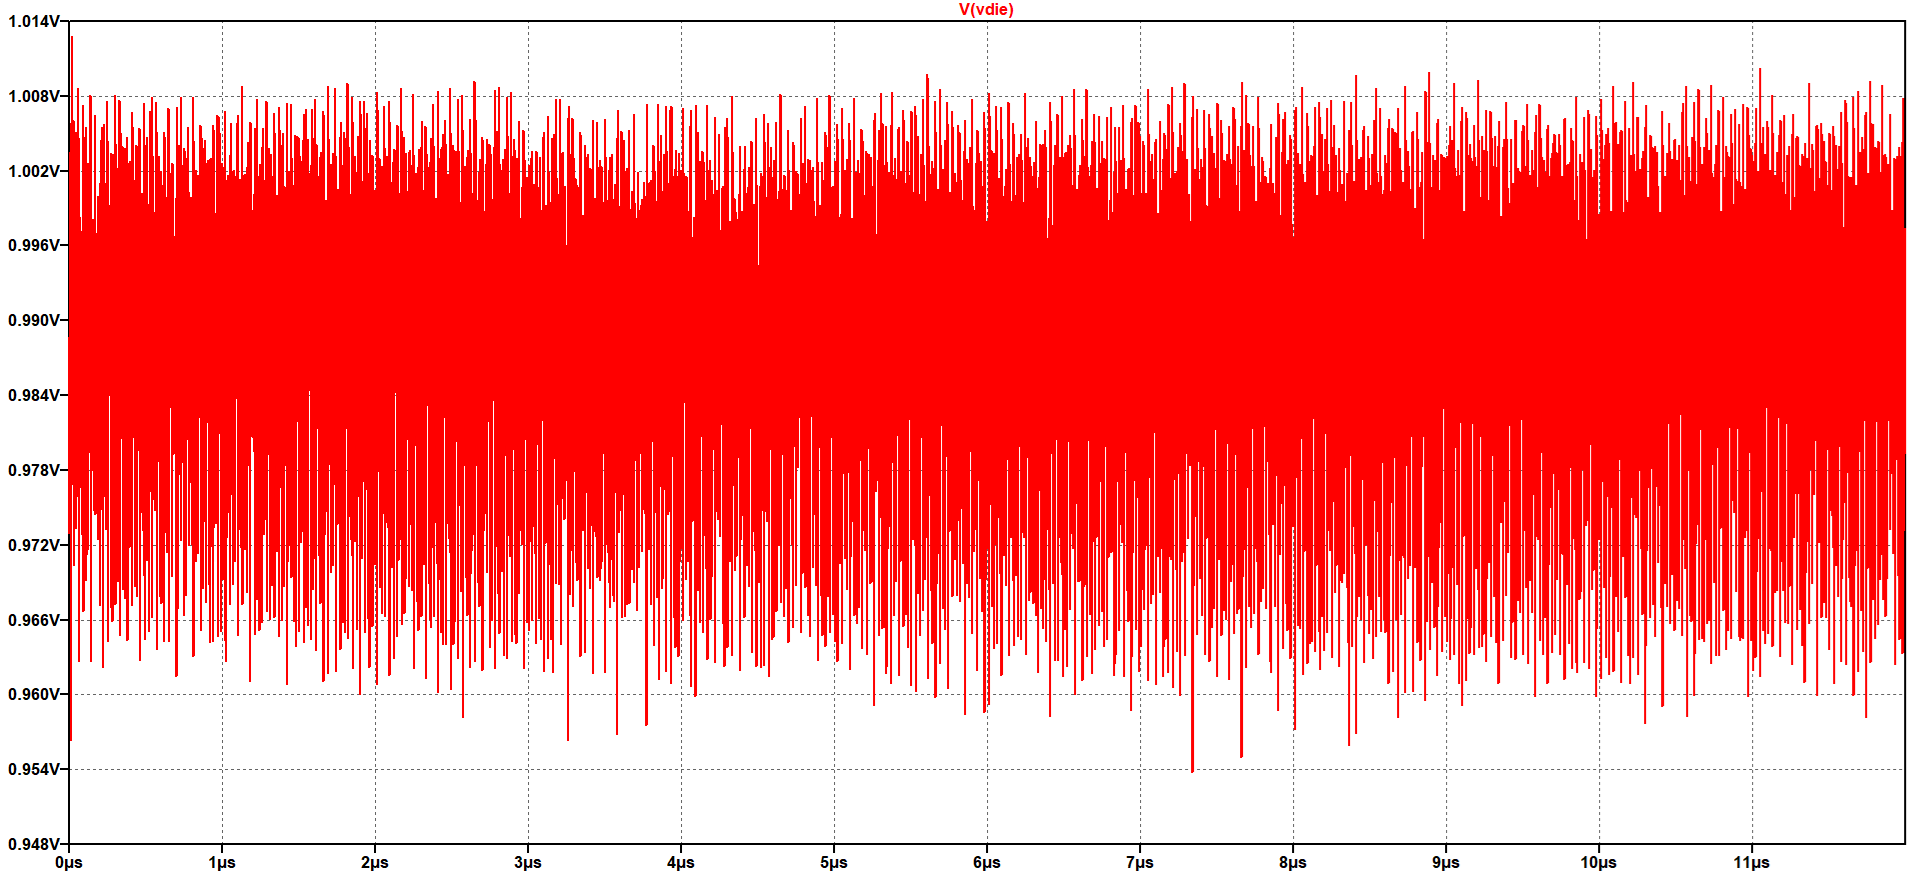
\includegraphics[width=\textwidth]{./eser5/vdie_best.png}
%\fbox{\parbox{0.9\textwidth}{\centering\vspace{3cm} Figure placeholder: $V(\texttt{vdie})$ with the optimal decoupling capacitors\vspace{3cm}}}
\caption{Voltage at the die interface with the optimal decoupling capacitors over the whole simulation ($12~\mu\text{s}$).}
\label{fig:vdie_best}
\end{figure}

\noindent The value predicted by the method, $57.6~\text{mV}$, is slightly lower than the one of the transient. This is expected: the method gives the periodic steady state, while the
transient simulation starts from the DC operating point and includes the start-up of the network, which adds a spike in the first tens of nanoseconds. For the PDN without decoupling capacitors this effect is negligible
($282.2~\text{mV}$ predicted, $280.8~\text{mV}$ simulated), because the ripple is much larger, but it is a few percent of the ripple with the optimal capacitors.
% TODO: if the ripple is measured excluding the start-up (.meas tran vpp_ss PP V(vdie) FROM=0.5u TO=12u), write here the value and say that it is closer to the prediction.

\begin{table}[!h]
\centering
\caption{Comparison between the PDN without decoupling capacitors and with the optimal configuration.}
\label{tab:comp_best}
\begin{tabular}{lcc}
\hline
 & \textbf{No decaps} & \textbf{Optimal decaps} \\
\hline
$\max |Z_{die}|$ [$\Omega$]                          & 3.06 & 0.8286 \\
Frequency of the maximum [MHz]                       & 95.9 & 74.918 \\
$|Z_{die}|$ at 100~MHz [$\Omega$]                    & 2.05 & 0.1702 \\
$V_{pp}$ from the method [mV]                        & 282.2 & 57.6 \\
$V_{pp}$ from the transient (LTspice) [mV]           & 280.8 & 59.5 \\
\hline
\end{tabular}
\end{table}

%%%%%%%%%%%%%%%%%%%%%%%%%%%%%%%%%%%%%%%%%%%%%%%%%%%%%%%%%%%

\subsection{Comparison with other configurations}

To evaluate the benefit of the optimisation, the optimal configuration is finally compared with the PDN without decoupling capacitors and with the six configurations that
use the same capacitor on all the five locations. \autoref{tab:comp_all} collects the impedance and the ripple: the values from the method of \autoref{sec:theory} are
reported together with the ones of the direct LTspice transient simulation.

\begin{table}[!h]
\centering
\caption{Comparison of the configurations. The ripple of the transient simulation is the \texttt{.meas} of LTspice over the whole simulation.}
\label{tab:comp_all}
\begin{tabular}{lcccc}
\hline
\textbf{Configuration} & $\max|Z_{die}|$ [$\Omega$] & $|Z_{die}|_{100~\text{MHz}}$ [$\Omega$] & $V_{pp}$ method [mV] & $V_{pp}$ LTspice [mV] \\
\hline
No decaps             & 3.06 (95.9~MHz)  & 2.05  & 282.2 & 280.8 \\
$5\times$ 10~nF       & 1.86 (120.4~MHz) & 0.443 & 96.5  & --  \\
$5\times$ 6.8~nF      & 1.59 (122.7~MHz) & 0.368 & 83.4  & --  \\
$5\times$ 4.7~nF      & 1.27 (125.3~MHz) & 0.298 & 74.0  & --  \\
$5\times$ 3.3~nF      & 0.894 (131.6~MHz)& 0.173 & 64.0  & --  \\
$5\times$ 2.2~nF      & 0.837 (75.3~MHz) & 0.176 & 60.1  & --  \\
$5\times$ 1.5~nF      & 1.23 (81.1~MHz)  & 0.336 & 86.7  & --  \\
Optimal               & 0.829 (74.9~MHz) & 0.170 & 57.6  & 59.5 \\
\hline
\end{tabular}
\end{table}
% TODO: fill the last column with the .meas results of the six LTspice transient simulations with the same capacitor on the five locations.
% TODO: comment the final table after the simulations: the values of the method are already in the table, they should be confirmed by LTspice.

\noindent With the same capacitor on all the locations, the ripple does not decrease with the capacitance: the five 10~nF capacitors, the largest ones, give the highest ripple among the
configurations with decoupling capacitors, $96.5~\text{mV}$, while the lowest ripple of this group is obtained with $5\times 2.2~\text{nF}$, $60.1~\text{mV}$. In all cases the capacitors reduce the ripple with respect to the
PDN alone by a factor of about three or more. The optimal configuration, which mixes capacitors with different self-resonance frequencies, gives the lowest ripple of all, but its advantage over the best uniform
configuration is small, about $4\%$: the improvement of the optimisation comes mainly from the choice of the right values, and only marginally from their distribution among the five locations.


%\noindent\\ However, all the measurements described above are taken inside the whole simulation window, so they include the initial transient,
%when the voltage is still settling from 0~V to its steady-state value. In order to have a more realistic evaluation of the ripple,
%the first 0.5~$\mu$s of simulation should be excluded, so only the last 11.5~$\mu$s are really significant for the ripple evaluation.
%In this way, all measurements are performed when the voltage has already settled to its steady-state behaviour.\\ As a consequence, a less pessimistic
%scenario is obtained (see last column of \autoref{tab:ripple}), but the measured ripple is still critical, equal to  peak-to-peak, which is  of the supply voltage, and the voltage still goes below 0.95~V and above 1.05~V.